\documentclass[tikz,border=8pt]{standalone}
% Requer xelatex e a fonte Poppins. Ajuste o Path abaixo (ou use \setmainfont{Poppins} se ela estiver instalada).
\usepackage{fontspec}
\setmainfont{Poppins}[Path=/usr/share/fonts/truetype/google-fonts/,Extension=.ttf,UprightFont=*-Regular,BoldFont=*-Bold,ItalicFont=*-Italic,BoldItalicFont=*-BoldItalic]
\usepackage{xcolor}
\definecolor{azulescuro}{HTML}{4A6F9C}
\definecolor{azulmedio}{HTML}{6F93BC}
\definecolor{azulclaro}{HTML}{E9EDF3}
\definecolor{azulsenac}{HTML}{1F4E9A}
\definecolor{laranja}{HTML}{F19E37}
\definecolor{laranjaescuro}{HTML}{D9731A}
\definecolor{laranjaclaro}{HTML}{FDEFD9}
\definecolor{cinzatitulo}{HTML}{333333}
\definecolor{cinzatexto}{HTML}{5C5C5C}
\usepackage{tikz}
\usetikzlibrary{positioning,arrows.meta,fit,backgrounds,calc}

\definecolor{vazio}{HTML}{EEF1F6}
\newcommand{\ok}[1]{\draw[white, line width=1.6pt, line cap=round, line join=round] ($(#1)+(-0.17,-0.01)$) -- ($(#1)+(-0.05,-0.14)$) -- ($(#1)+(0.18,0.15)$);}
\newcommand{\nao}[1]{\draw[azulmedio!70, line width=1.2pt, line cap=round] ($(#1)+(-0.13,-0.13)$) -- ($(#1)+(0.13,0.13)$) ($(#1)+(-0.13,0.13)$) -- ($(#1)+(0.13,-0.13)$);}
\begin{document}
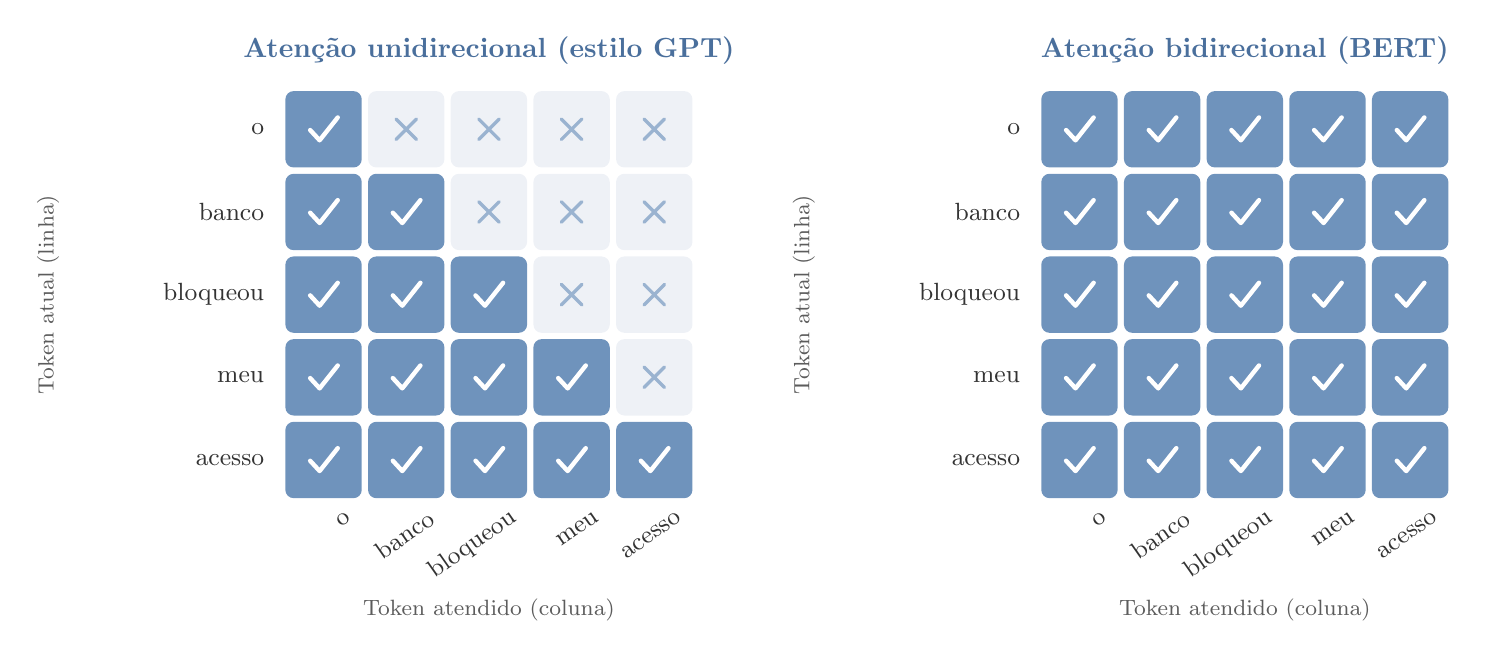
\begin{tikzpicture}[font=\small\color{cinzatexto}]
\def\s{1.05}
\def\pal{{"o","banco","bloqueou","meu","acesso"}}
\foreach \m/\ox/\tit/\causal in {0/0/{Atenção unidirecional (estilo GPT)}/1, 1/9.6/{Atenção bidirecional (BERT)}/0}{
  \foreach \i in {0,...,4}{
    \foreach \j in {0,...,4}{
      \pgfmathtruncatemacro{\perm}{\causal==0 ? 1 : (\j<=\i ? 1 : 0)}
      \coordinate (c) at (\ox+\j*\s, -\i*\s);
      \ifnum\perm=1
        \fill[azulmedio, rounded corners=3pt] ($(c)+(-0.5*\s+0.04,-0.5*\s+0.04)$) rectangle ($(c)+(0.5*\s-0.04,0.5*\s-0.04)$);
        \ok{c}
      \else
        \fill[vazio, rounded corners=3pt] ($(c)+(-0.5*\s+0.04,-0.5*\s+0.04)$) rectangle ($(c)+(0.5*\s-0.04,0.5*\s-0.04)$);
        \nao{c}
      \fi
    }
    \node[anchor=east, font=\small\color{cinzatitulo}] at (\ox-0.6*\s,-\i*\s) {\pgfmathparse{\pal[\i]}\pgfmathresult};
    \node[anchor=east, rotate=35, font=\small\color{cinzatitulo}, inner sep=1pt] at (\ox+\i*\s+0.35,-4*\s-0.65*\s) {\pgfmathparse{\pal[\i]}\pgfmathresult};
  }
  \node[font=\normalsize\bfseries\color{azulescuro}] at (\ox+2*\s,0.95*\s) {\tit};
  \node[rotate=90, font=\footnotesize\color{cinzatexto}] at (\ox-3.5,-2*\s) {Token atual (linha)};
  \node[font=\footnotesize\color{cinzatexto}] at (\ox+2*\s,-4*\s-1.9) {Token atendido (coluna)};
}
\end{tikzpicture}
\end{document}
